\begin{refsegment}
\chapter{GROOLS}

J'ai consacré ces trois années de recherche pour une approche interactive entre le biologiste et les prédictions bio-informatiques lors du processus de curation de l'annotation fonctionnelle des génomes bactériens. Compte tenu de l'augmentation constante et rapide des annotations automatiques, un système expert pourrait assister les biologistes à détecter les annotations inconsistantes et contradictoires. La curation et la validation des prédictions bio-informatiques pourrait alors rattraper se retard.

\section{Le début de GROOLS}

\subsection{HERBS}

L'équipe \texttt{HELIX} d'\textit{Alain VIARI} avait commencé un projet en ce sens nommé \texttt{\gls{HERBS}} en collaboration avec le \texttt{\gls{SIB}} dans le cadre du projet \gls{HAMAP} \cite{pedruzzi2015hamap}. L'objectif de \texttt{\gls{HERBS}} est d'alerter les biologistes sur les voies métaboliques manquantes, non attendues ou encore ambiguës. Pour cela l'outil s'appuie sur un moteur d'inférence \texttt{\gls{JESS}}, d'une base de connaissance (contenant les règles et les faits, \cref{fig:systeme_expert}) et d'une interface graphique pour l'exploration des connaissances. \textit{Alain VIARI} m'a permis d'utiliser l'outil \texttt{PathRules} qui est une implémentation de \texttt{\gls{HERBS}} avec le moteur \texttt{\gls{CLIPS}} \cite{riley1991clips}.


J'ai fournis à la base de fait de  \texttt{PathRules} les voies de biosynthèse de la lysine (AAA et DAP) décrit par \texttt{UniPathway} et les prédictions provenant de 79 organismes. Pour ce faire les données sont rangées dans trois dossiers présent à la racine du projet: (i) "data/processes" pour la description des voies métaboliques, (ii) "data/observers/uniprot" pour le catalogues des prédictions par espèces, (iii) "data/species" pour la description taxonomique des espèces. Les fichiers doivent porter l'extension \texttt{.data} et le nom du fichier est utilisé comme identifiant pour faire le lien entre les processus, les prédictions et les informations taxonomiques de l'espèce. Par exemple, j'ai utilisé l'identifiant ACIAD pour mettre en relation les informations d'\textit{Acinetobacter sp ADP1}.

\console{find data/ -name 'ACIAD.data'}{ data/observers/uniprot/ACIAD.data\par data/species/ACIAD.data }


La description des données dans ses fichiers suit la nomenclature \texttt{\gls{CLIPS}}. C'est à dire que les faits sont déclarés entre parenthèses. Les observations sont formatées comme suit: ( \texttt{source} (id \texttt{xxx}) (alias \texttt{yyy} sp:\texttt{zzz})  ) .

Extrait d'un fichier cataloguant les faits relatives à une espèce:\nolisttopbreak

\console{head data/observers/uniprot/data/ACIAD.data}{
    (uniprot (id ASPARTATE-SEMIALDEHYDE-DEHYDROGENASE-RXN) (alias ACIAD0479 sp:ACIAD00423))\par
    (uniprot (id SUCCDIAMINOPIMDESUCC-RXN) (alias ACIAD0791 sp:ACIAD0070)\par
    (uniprot (id ASPARTATEKIN-RXN) (alias ACIAD1252 sp:ACIAD01133))\par
    (uniprot (id SUCCINYLDIAMINOPIMTRANS-RXN) (alias ACIAD2080 sp:ACIAD01886))\par
    (uniprot (id TETHYDPICSUCC-RXN) (alias ACIAD2599 sp:ACIAD02357))\par
    (uniprot (id DIAMINOPIMEPIM-RXN) (alias ACIAD2659 sp:ACIAD02412))\par
    (uniprot (id DIAMINOPIMDECARB-RXN) (alias ACIAD2660 sp:ACIAD02413))\par
    (uniprot (id DIHYDRODIPICSYN-RXN) (alias ACIAD3585 sp:ACIAD03222))\par
    (uniprot (id DIHYDROPICRED-RXN) (alias ACIAD3619 sp:ACIAD03252))\par
}


L'information taxonomique est également un fait. Il débute par "species" suivis de plusieurs chaîne de caractères pour renseigné de plus en plus précisément la taxonomie de l'organisme.

\console{cat data/species/ACIAD.data}{ (species lineage Bacteria Proteobacteria Gammaproteobacteria Pseudomonadales Moraxellaceae Acinetobacter Acinetobacter\_sp.\_ADP1) }

Pour représenter la structure hiérarchique des voies métaboliques, les faits sont organisés pour exprimer la notion de composition et d'équivalence. La notion de composition et utilisé pour relier les blocs réactionnelles à leurs réactions. Quant à l'équivalence elle permet de définir les chemins alternatifs pour réaliser une voie métabolique. La syntaxe \texttt{\gls{CLIPS}} utilise $x -> \ldots$ pour signifier "x tel que \ldots". La partie à droite de la flèche décrit les relations en notation polonaise\footnote{Également connue sous le nom "notation pré-fixée". Par exemple, le calcul "$5 \times (2 + 3)$", s'écrit "$\times 5 (+ 2 3)$". }. Ci-après la voie métabolique de la biosynthèse de la lysine par la voie AAA (Acide Alpha-amino Adipique) selon \texttt{UniPathway}.

\console{cat data/processes/lysine\_AAA\_biosynthesis.data}{
;;;; --------------------------------------------------------\par
;;; HERBS (Hamap Expert Rules Based System)\par
;;;\par
;;; @file: lysine\_AAA\_biosynthesis.data\par
;;; --------------------------------------------------------\par
;;;\par
(process declare lysine\_AAA\_biosynthesis present in ALL)\par
(process define lysine\_AAA\_biosynthesis -> and UPA00033)\par
(process define UPA00033 -> or UPA00033-alt-0 UPA00033-alt-1)\par
(process define UPA00033-alt-0 -> and ULS00012 ULS00013)\par
(process define UPA00033-alt-1 -> and ULS00012 ULS00014)\par
(process define ULS00012 -> and ULS00012-alt-0)\par
(process define ULS00012-alt-0 -> and UER00028 UER00029 UER00030 UER00031 UER01027)\par
(process define ULS00013 -> or ULS00013-alt-0 ULS00013-alt-1)\par
(process define ULS00013-alt-0 -> and UER00032 UER00034)\par
(process define ULS00013-alt-1 -> and UER00033 UER00034)\par
(process define ULS00012 -> and ULS00012-alt-0)\par
(process define ULS00012-alt-0 -> and UER00028 UER00029 UER00030 UER00031 UER01027)\par
(process define ULS00014 -> or ULS00014-alt-0 ULS00014-alt-1)\par
(process define ULS00014-alt-0 -> and UER00035 UER00037 UER00038 UER00039)\par
(process define ULS00014-alt-1 -> and UER00036 UER00037 UER00038 UER00039)\par
}


Chaque processus est un fait désigné par le mot clé "process". Les voies métabolique sont préfixer du mot clé "declare" et "define" pour ces composants. Les faits constituant la voie métabolique sont hiérarchiquement organisé. Lorsque un fait et composé de plusieurs concepts on utilise le symbole "and" et "or" lorsqu'un fait possède des équivalences. Les lignes débutant par un point virgules ne sont pas interprété par  \texttt{\gls{CLIPS}}.

Ceci permet d'obtenir une évaluation de la complétion de l'annotation fonctionnelle des génomes (\cref{fig:herbs_rapport}).

\begin{shadedfigure}[H]
    \centering
    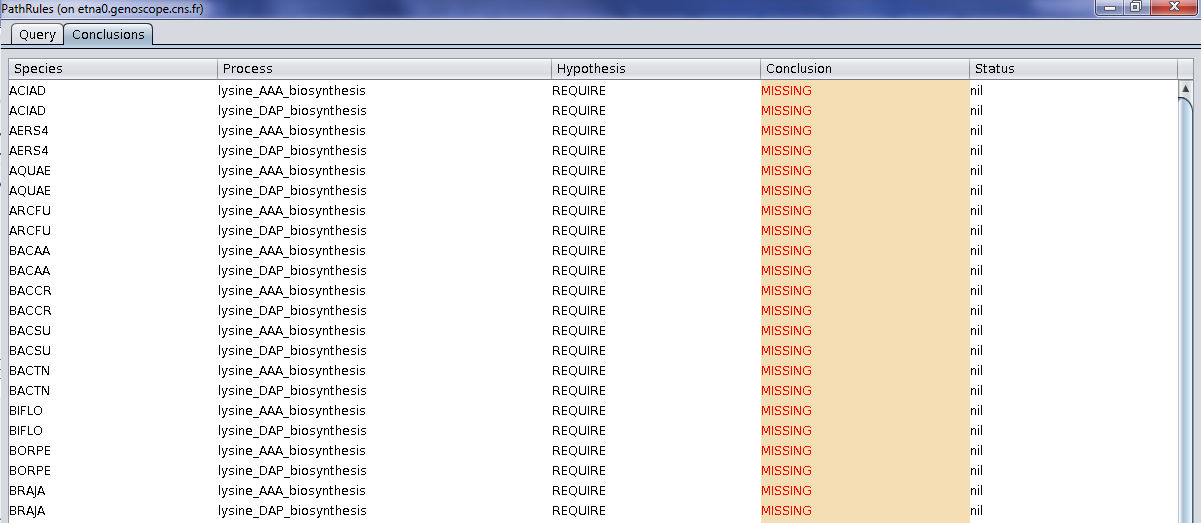
\includegraphics[width=\textwidth]{img/herbs_conclusion_report.png}
    \caption{Rapport sur la présence de la voie de biosynthèse de la lysine.}
    \label{fig:herbs_rapport}
\end{shadedfigure}

L'utilisateur à la possibilité d'explorer les voies métaboliques à travers le graphe orienté acyclique pour discriminer les composants du métabolisme manquants (\cref{fig:herbs_dag}).

\begin{landscape}
    \begin{shadedfigure}[H]
        \centering
        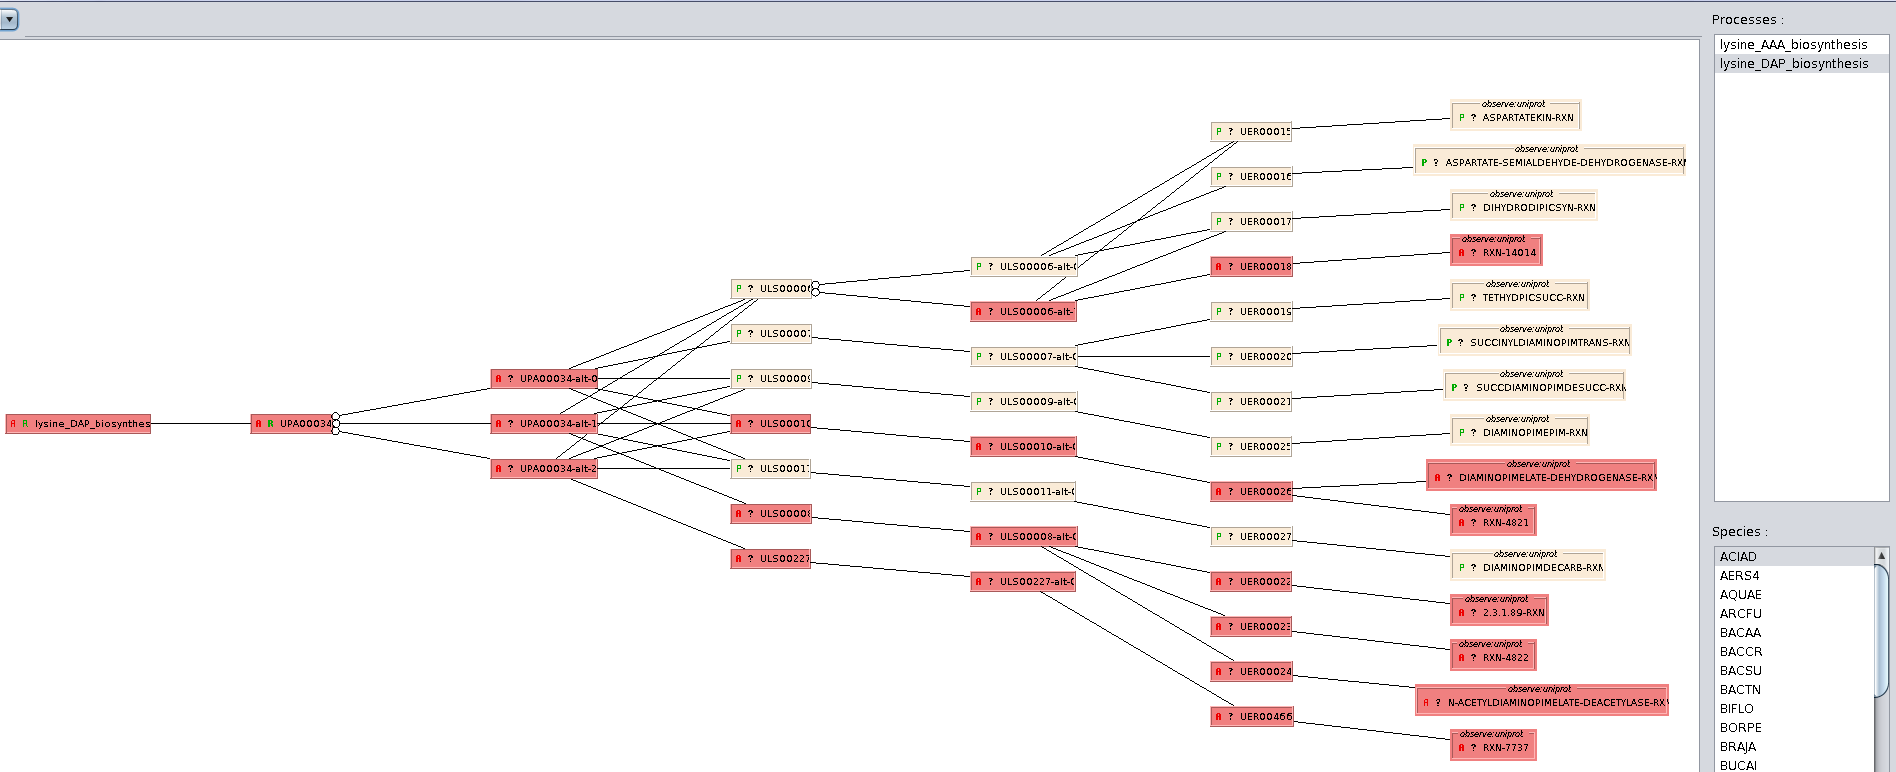
\includegraphics[width=\textwidth]{img/herbs_aciad_lysine_dap.png}
        \caption{Rapport sur la présence de la voie de biosynthèse de la lysine.}
        \label{fig:herbs_dag}
    \end{shadedfigure}
\end{landscape}


Pour passer à l'échelle, il est nécessaire de retranscrire  en \texttt{\gls{CLIPS}}  toutes les voies métaboliques et toutes les prédictions bio-informatiques. De plus le système doit être étendue à la notion d'inconnu et si possible à la notion de contradiction. Car en biologie, nous possédons la connaissance de ce qui est et ce qui n'est pas présent, pour le reste nous n'avons pas d'idée. Ce point de vue, peut paraître un peu philosophique. Il fait référence aux concepts de "monde ouvert" et "monde fermé". Une hypothèse en monde fermé va considéré toutes les questions sans réponses comme fausses. En monde ouvert, les hypothèses prennent les valeurs vrais ou fausses lorsqu'elles sont explicitement décrites comme telles. Pour les autres cas les hypothèses sont considérés incertaines tant qu'un fait ne la désigne pas comme vrai ou fausse. Dans le cas présent la plupart des voies métaboliques sont déclarés "MISSING" ce qui n'aide pas beaucoup le biologiste. Ceci est dues au raisonnement en monde fermé, en biologie quantité de connaissances ne sont pas prédites et pour autant cela ne signifie pas qu'elles sont prédites comme non présentes dans l'organisme.

\subsection{GROOLS: Un système à base de règle pour l'annotation fonctionnelle des génomes microbiens}

Mon projet de recherche débute par l'identification des besoins et des outils à ma disposition. Les besoins de la plateforme se divise en trois axes.

Le premier  corresponds à la modernisation du système de gestion et déclaration des chaînages applicatifs. Pour cela la plateforme MicroScope s'oriente par la mise en place du moteur pour le chaînage d'application à base de règle développé en interne au GenoScope (\texttt{\gls{BIRDS}}) . Le système utilise l'application \texttt{DROOLS}\cite{browne2009jboss} pour raisonner et donc ordonnées les processus. Il est donc nécessaire d'informé à \gls{BIRDS} comment organiser les processus de l'annotation.

Le second axe consiste à pourvoir discuter avec le  système d'intégration continue des donnée interne à la plateforme, dénommé Galileo \cite{galileo2014}. Cet outil à la faculté de réconcilié les informations provenant de multiple ressource interne et donc d'avoir accès à un large éventail d'information à travers une unique interface. Ceci lui permet de fournir une représentation unifié des voies métaboliques par l'utilisation des information de \texttt{CHebi}, \texttt{RHEA}, \texttt{KEGG} et \texttt{MetaCyc}.

Le troisième axe s'articule autour d'un système à base de règle pour l'annotation des génomes et guider le biologiste sur les annotations suspecté manquante dans un organsine donnée. Il est composé de deux sous partie. La première a pour objectif de récupérer les règles d'UniRule et de les rendre utilisable en dehors de "l'\gsl{EBI}". Les règles d'annotation fonctionnelles à partir des domaines protéiques seraient ainsi partagé à la communauté scientifique. La deuxième partie se consacre à la mise en évidence des régions de connaissances non prédites ou contradictoire. La cohérence des génomes peut être évalué au regards des attentes porté sur les fonction des organismes. L'application \texttt{DROOLS} a été choisie pour la mise en œuvre du raisonnement afin de garder la maitrise autour d'une même application pour tout développement impliquant un système à base de règle. Cet application se montre moderne et capable de communiquer avec les application java ce  qui est un avantage car Galileo est écrit en Java.

C'est sur ce dernier axe que j'ai effectué mes recherches tout en échangeant sur les deux premiers axes afin de récupérer les prédictions bio-informatiques et les voies métaboliques unifié. Le cadre de mon projet de recherche a été présenté lors de la 10$^{eme}$ conférence international sur l'intégration de donnée en science de la vie (DILS 2014 \url{http://dils2014.inesc-id.pt/}).

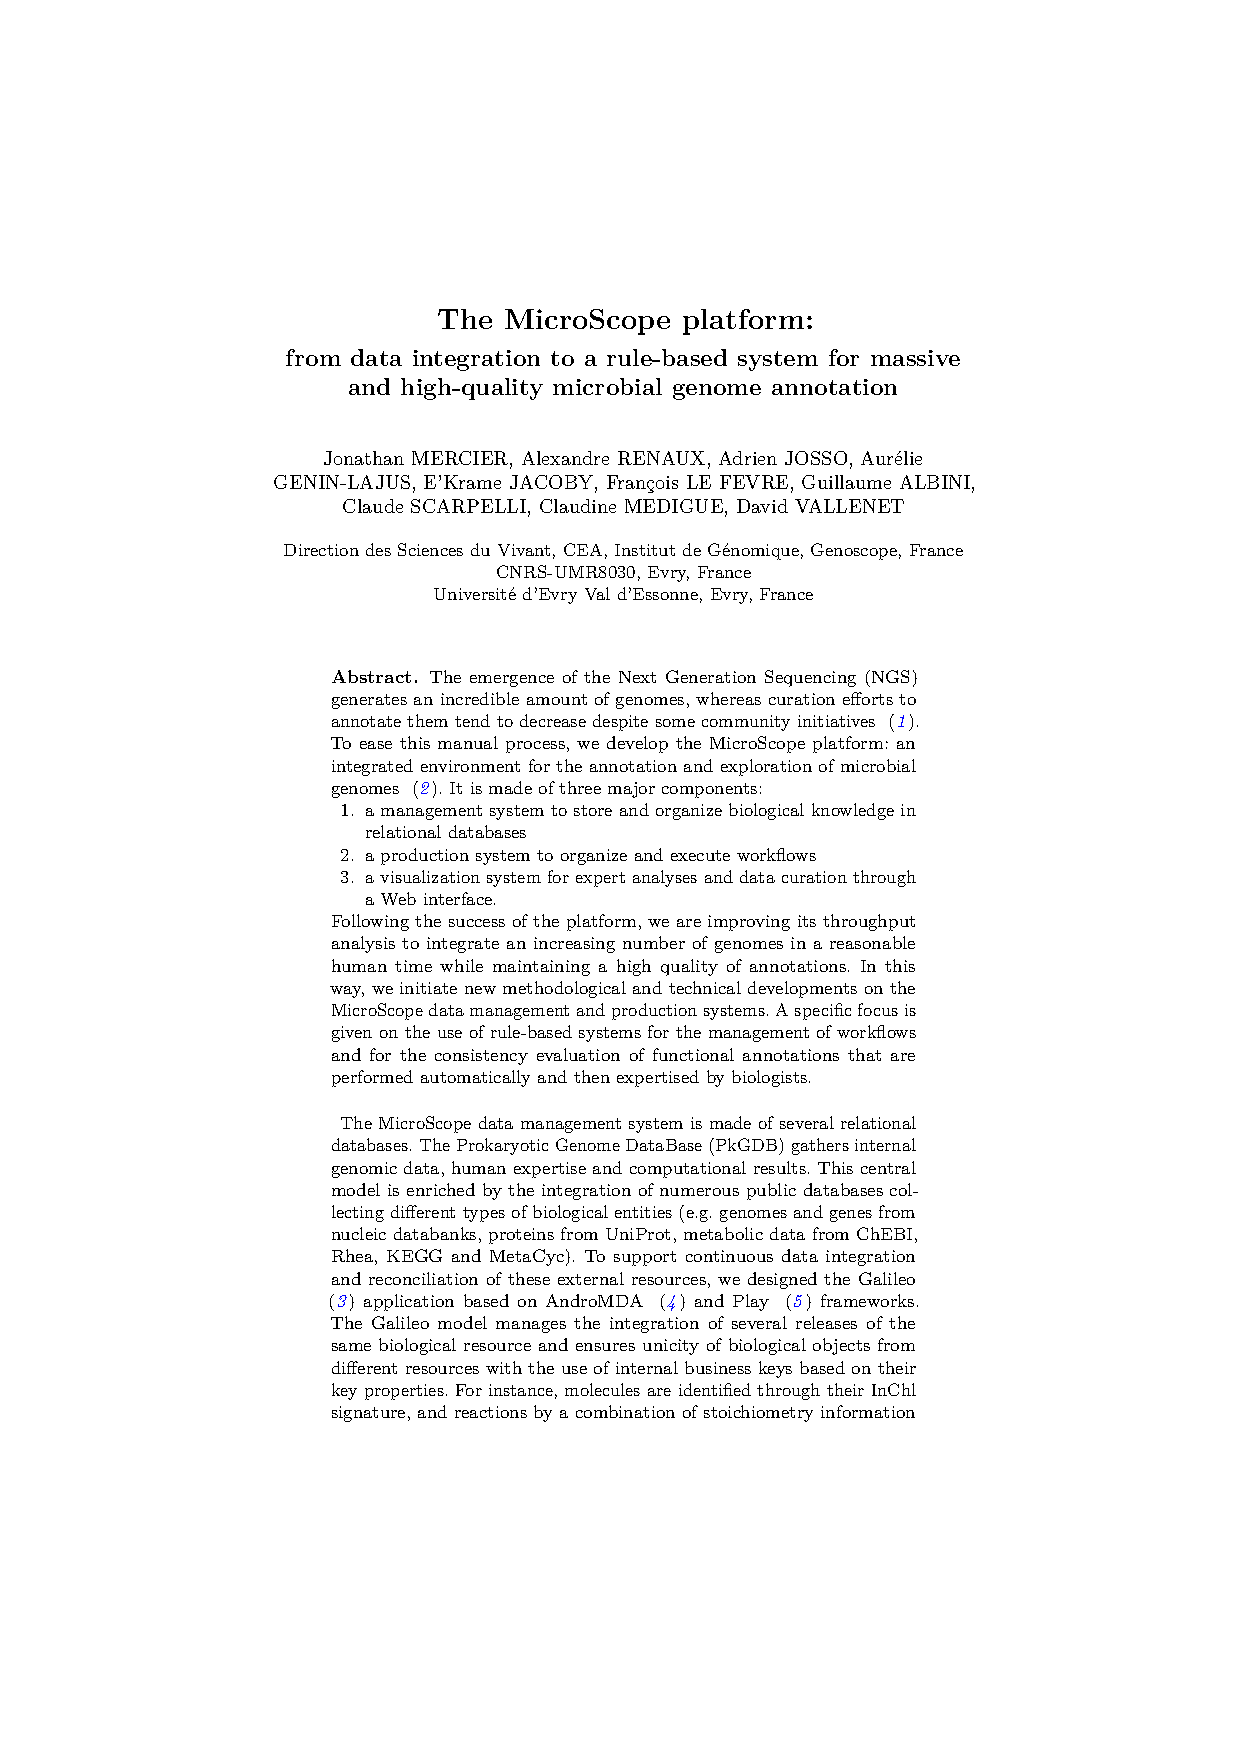
\includepdf[pages=-]{img/DILS_2014.pdf}

\subsection{Investigation sur les règles de logiques}

Au début de mes investigations, j'ai rencontré plusieurs difficultés. La première était d'utiliser les données structurées et complexes issues de la biologie à travers des règles de logique. Il faut savoir que la plupart des raisonneurs (comme \texttt{Prolog} et \texttt{CLIPS}) utilise la programmation déclarative, ce qui consiste à décrire le problème\footnote{Par opposition a des langages comme Java, Python, D, Perl \ldots, ils utilisent la programmation impérative qui s'attache à décrire comment trouver la solution.}. La déclaration de problème impliquant  des données structurées n'était pas initialement prévue dans ce paradigme\footnote{Des extensions du paradigmes ont permis de gérer des structures de données complexes comme Prolog++.}. Par exemple un bloc de réaction  composé de la réaction A et B peut s'exprimer par la règle suivante (en Prolog):

\begin{lstlisting}[basicstyle=\small\normalfont\ttfamily,language=Prolog]
    reaction_block(Arg1, Arg2) :-
        reaction_A(Arg1),
        reaction_B(Arg2).
\end{lstlisting}

Ce qui précède  ":-" est le nom de la règle et ces arguments, ce symbole signifie "si". Pour reprendre l'exemple précédant "reaction\_block(Arg1,Arg2)" est vrai si "reaction\_A(Arg1)" et "reaction\_B(Arg2)" sont vrais. Il n'est pas simple de rattaché des attributs à des catégories de réaction comme on pourrait le faire avec le paradigme orienté-objet. C'est la raison pour laquelle j'ai utilisé le système \texttt{DROOLS}. Il permet d'utiliser des objets (au sens Java)  et de les utiliser pour établie des règles. Par exemple l'utilisation d'un attribut peut être employé pour indiquer que certaines réactions sont optionnel et ainsi "relacher" la définition du bloc de réaction. Le raisonnement est influé par les états des différents attributs attaché à une réaction. Je devais donc établir un raisonnement utilisant des structures de données et leurs relations. Pour cela je me suis inspiré de "\citetitle{amir1999object}" \cite{amir1999object} et appuyé sur le projet \texttt{DROOLS} \cite{mcwhirter2001drools} pour écrire les règles de raisonnement et établir une description formelle des objets manipulé.

\subsection{La représentation des connaissances}

La seconde problématique portait sur la représentation des connaissances. Les voies métaboliques sont représentées de différentes manières selon la ressource utilisé. Il était nécessaire d'avoir un modèle hiérarchique des connaissances unifier pour utiliser indifféremment le même raisonnement. Pour cela, j'ai utilisé les représentations des voies métaboliques de \texttt{Metacyc} (\cref{fig:metacyc_lysine}), \texttt{KEGG} (\cref{fig:kegg_lysine}) et \texttt{Unipathway} (\cref{fig:lysine}) et recherché les caractéristiques pouvant être mise en commun. Cette étude a permis de mettre en place une structuration hiérarchiques de connaissance-apriori. Les observations sont reliées a ces connaissances-aprioris pour indiquer les attentes et les prédictions de ces dernières. Les observations et les connaissances-apriori sont des faits reliés les uns aux autres par des relations pour exprimer la composition et l'équivalence. Pour cela les opérateurs ET/OU sont employés pour exprimer ces deux notions et établir un raisonnement.

\begin{lstlisting}[basicstyle=\tiny\normalfont\ttfamily,caption=Inférence de la prédiction d'absence]
rule "Prediction infer his none existence"
when
    $k: Knowledge( $kid := id, nodeType == NodeType.LEAF )
    (
        or
        not( Prediction( $kid := knowledgeId ) )
        Prediction( $kid := knowledgeId, presence == FourState.UNKNOWN )
    )
then
    modify( $k ){
    presence = FourState.UNKNOWN
    }
end
\end{lstlisting}

\subsection{Gestion de l'incertitude et de la contradiction}

Quant à la troisième problématique, elle consistait à trouver la méthode logique pour travailler sur des données incertaines et incohérentes. Or la plupart des raisonneurs ( comme \texttt{CLIPS}, \texttt{PROLOG} \ldots ) s'inspire fortement la logique classique pour l'inférence des valeurs de vérité. Nous pensions qu'une telle problématique à forcément aboutis à une méthodologie applicable pour notre domaine d'étude. Cependant la grande majorité des raisonneurs ne proposaient pas un cadre pour l'utilisation de logique multi-valuées. Les valeurs vrai et fausse donne dans les système classique faux alors que nous souhaitions obtenir une valeur pour exprimer la contradiction. De même lorsqu'il y a aucun fait, la logique classique donne faux alors que la aussi nous souhaitions distinguer ce qui est  considéré comme faux de l'incertain. Pour cela mon travail de recherche ces basé sur les quatre valeurs de vérité décrites par \citeauthor{belnap77}\cite{belnap77}. J'ai établis une méthode pour le calcul des prédicats selon les opérateurs "ET" et "OU" dans un graphe de connaissance (\cref{fig:four_truth_values}). L'idée est d'inférer la valeur de vérité qui minimise l'incohérente à partir  d'un groupe de concepts enfant vers un concept parent. Cet approche s'apparente à un algorithme minmax \cite{aho1989} (\url{https://fr.wikipedia.org/wiki/Algorithme_minimax}). Par exemple dans le calcul: $ True \land Unknown \land False \to None$; le résultat est incertain car au moins un des concepts est ni-vrai-ni-faux par conséquent c'est la valeur utilisée pour l'inférence de la présence du groupe de concept vers le concept parent. Les règles de priorité pour l'inférence des valeurs de vérité étaient un moyen de retranscrire les tables de vérité de Belnap (présenté précédemment dans la partie \nameref{par:logic_multivalued} \cref{tab:belnap_truth_table}) dans des règles logiques.

\begin{shadedfigure}[H]
    \centering
    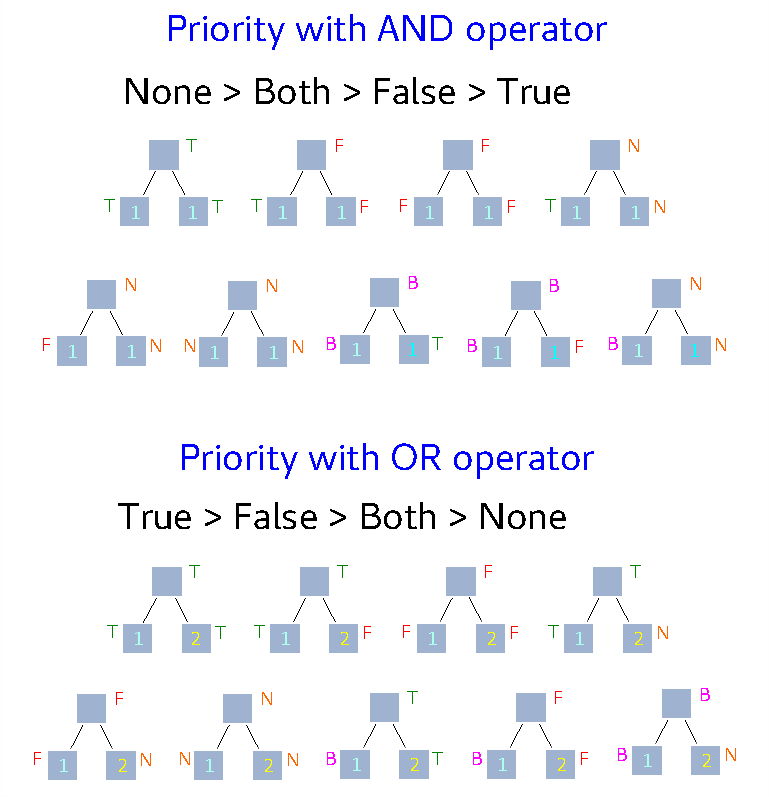
\includegraphics[width=\textwidth]{img/four_values_priorities_rules.pdf}
    \caption{ Règle de priorité pour l'inférences de multiple valeurs de vérité à travers un graphe "et/ou". }
    \label{fig:four_truth_values}
\end{shadedfigure}

La mise bout à bout des éléments précédemment cités permet d'écrire des règles

Ce travail à aboutis sur une première implémentation et présenté lors de la conférence \texttt{RULEML2015}.

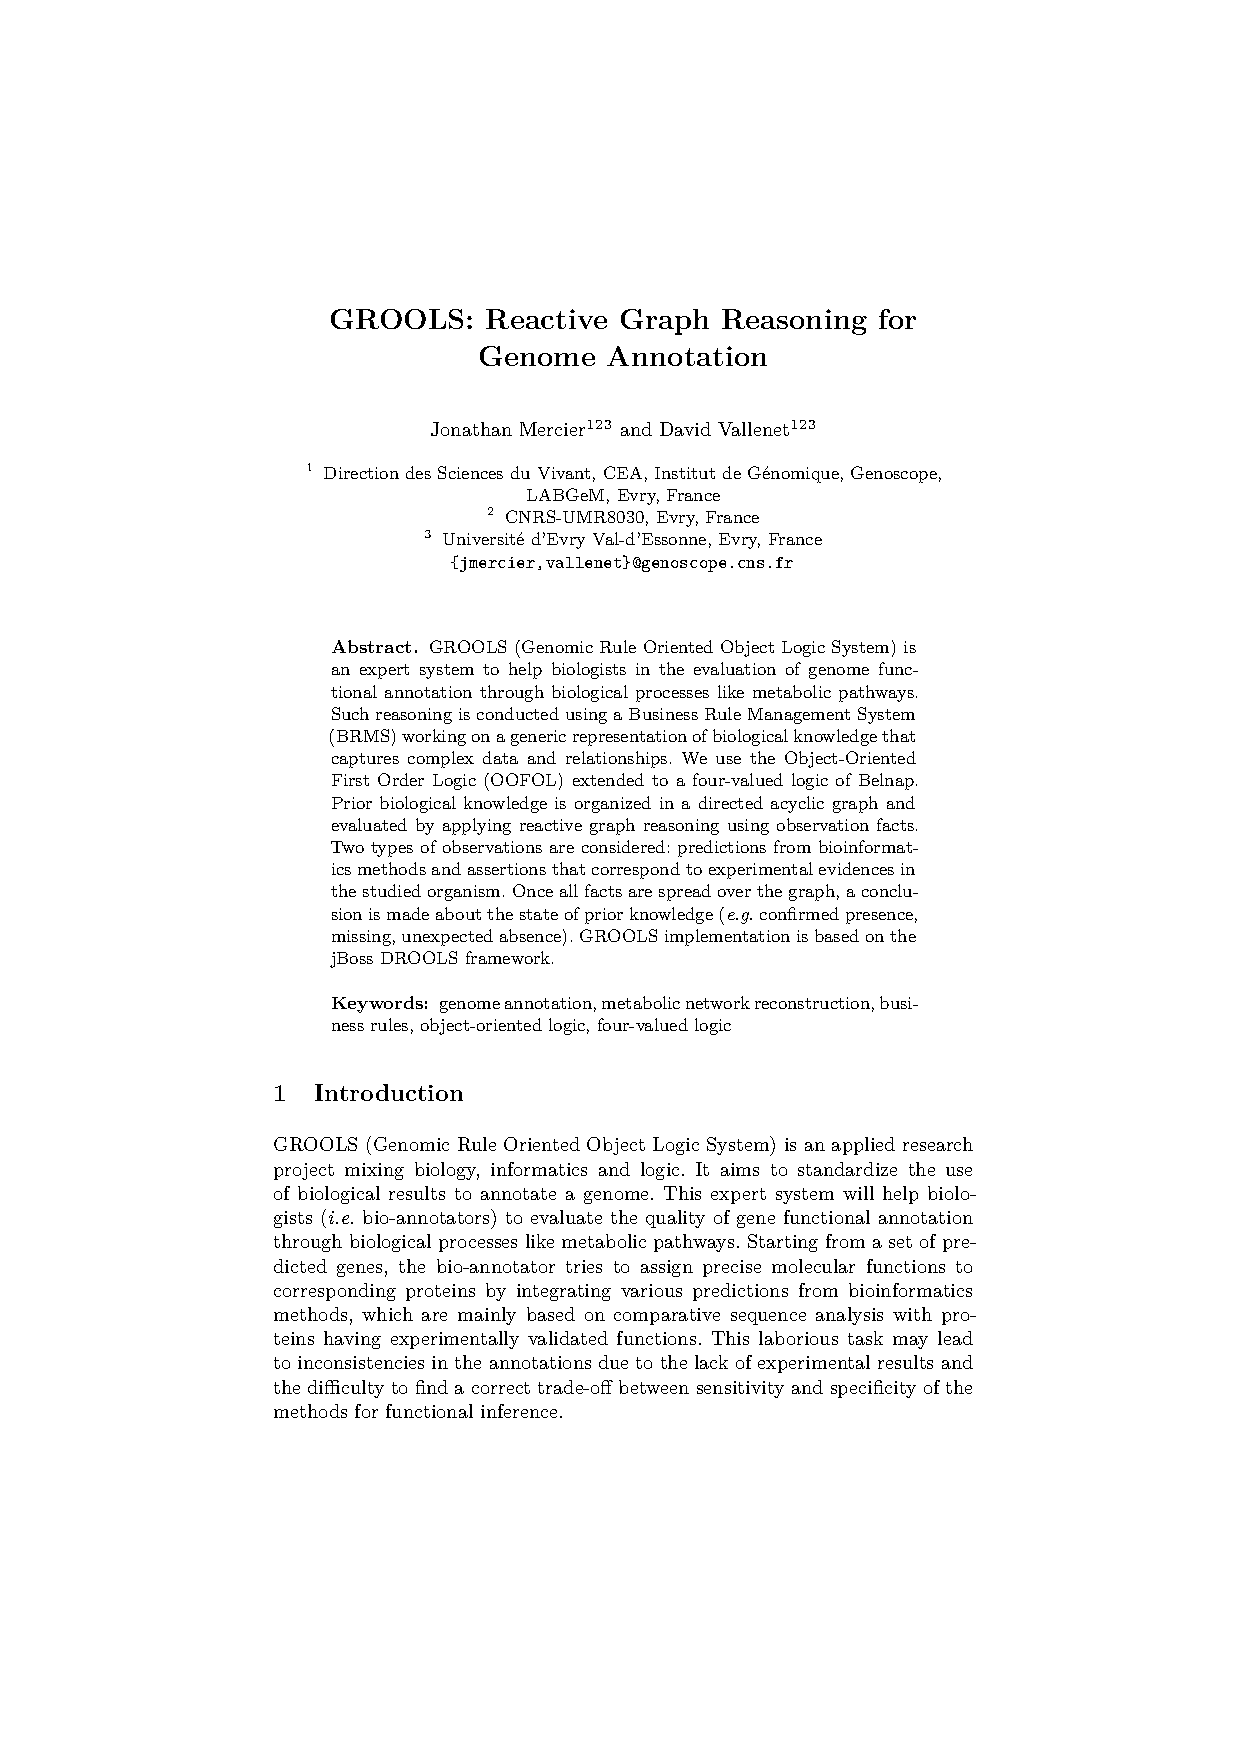
\includepdf[pages=-]{img/GROOLS__Reactive_Graph_Reasoning_for_Genome_Annotation.pdf}



La seconde est la contradiction
, de révéler les zones de connaissances couvertes par aucune prédiction et identifier les observations contradictoire.

expliqué les ratés
inaptitude à tout programmer de manière explicite

\textbf{Ce qui suit doit/peut être déplacé en discussion.}

Toutefois la méthode utilisé reste assez flou d'un point de vue formel. La distinction entre prédiction et expectation s'entre mêle. La combinaison de deux états (provenant de : certifié, inconnu, non certifié) implique neuf combinaisons possibles. Mais ces combinaisons sont représentables uniquement par les valeurs vrai,faux,inconnu. Donc un même résultat peut correspondre à plusieurs combinaisons possible. Ce qui amène à des phrases pour le moins subtile, par exemple la distinction entre inconnu et non certifié:
\begin{itemize}
    \item "The status “unknown” is assigned to an IMG pathway, in which IMG terms without gene assignments have “candidate genes”."
    \item "In contrast, the status “not asserted” is assigned to an IMG pathway when no “candidate genes” can be found."
\end{itemize}

De plus la notion de consistance est employé ici pour décrire un cadre logique. Mais en logique ce terme est utilisé pour désigné une chose ne contenant pas de contradiction. Or ici elle est utilisé abusivement pour décrire "une cohérence biologique".

Pour finir contrairement à leur constat sur les données biologiques erronées et donc la nécessité d'automatiser un raisonnement pour l'annotation fonctionnelle. Leur méthode aura pour tendance d'attribuer pour un génome partielle ou distant des génomes de références à une majorité d'états non certifiés ou inconnu. En conséquence les bio-curateurs seront difficilement plus aider par l'apport de ces nouvelles informations.


7 valeurs de vérité mais pas encore l'utilisation de l'ensemble vide


\section{Vers un raisonnement descriptif}
ensembliste valeur de vérité généralisé



\begin{shadedfigure}
    \centering
    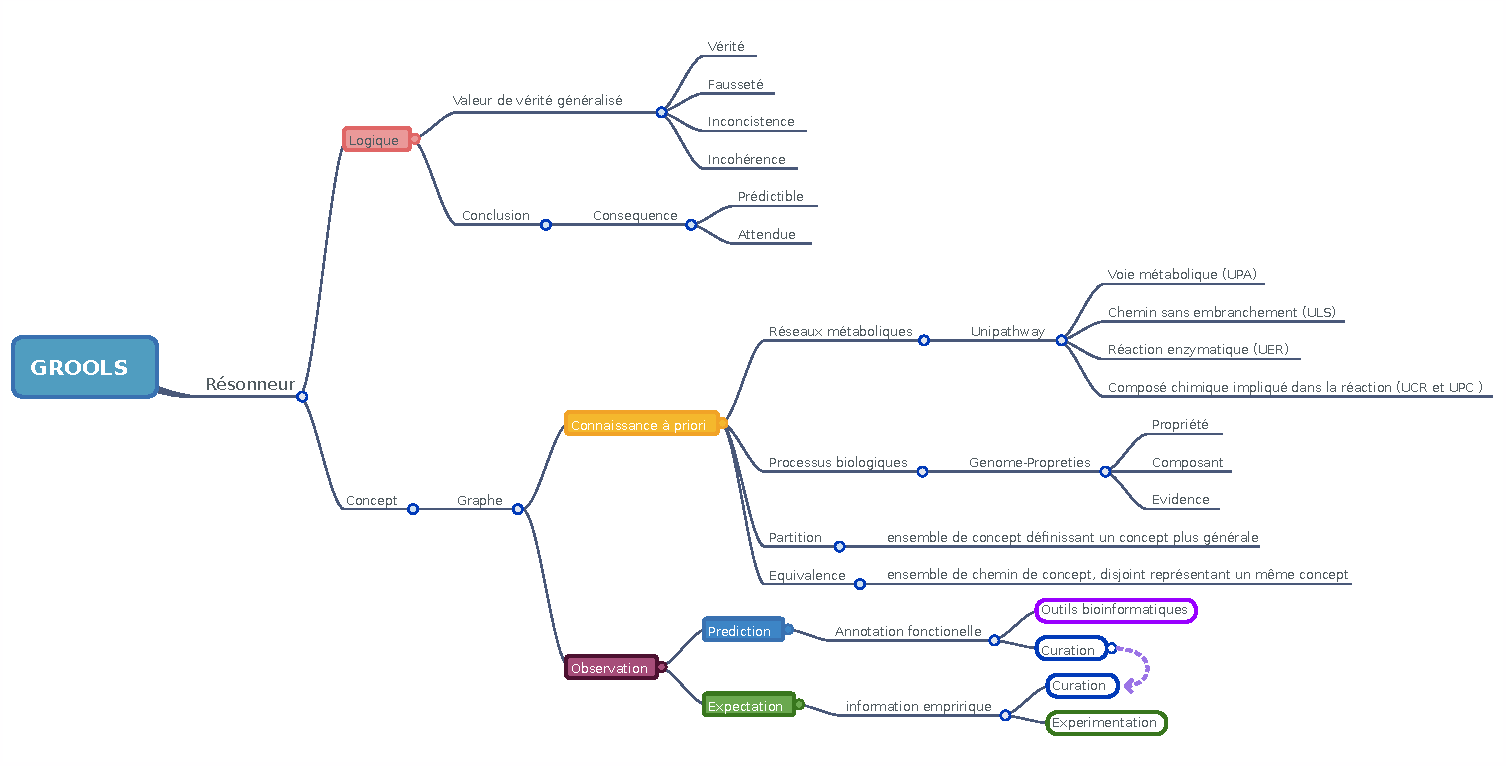
\includegraphics[width=\textwidth]{img/GROOLS_mindmap.pdf}
    \caption{  }
    \label{fig:GROOLS_mindmap}
\end{shadedfigure}

\section{La méthode}
le papier
pdf ici

discussion

\begin{shadedfigure}
    \centering
    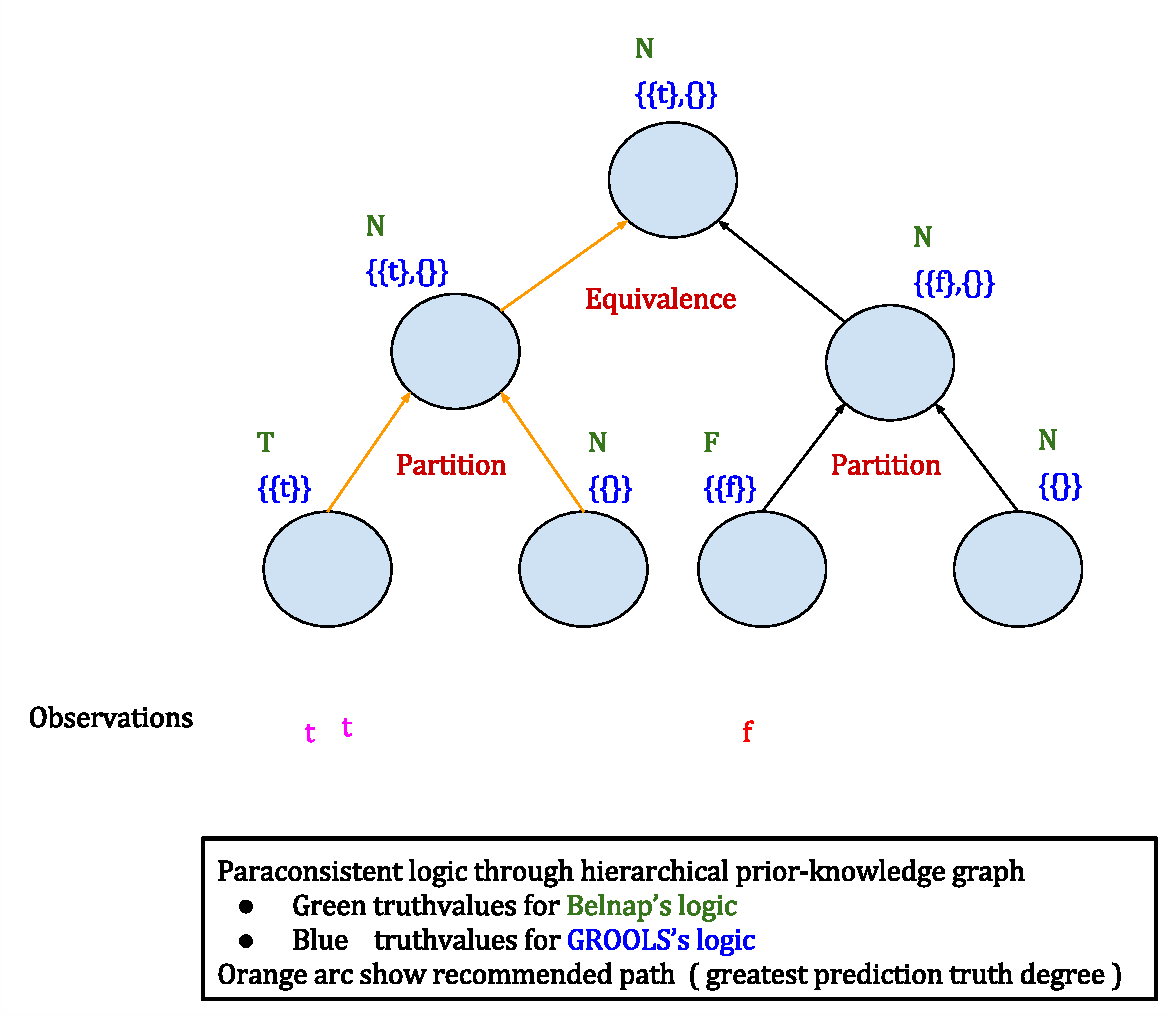
\includegraphics[width=\textwidth]{img/GROOLS_vs_belnap_1.pdf}
    \caption{  }
    \label{fig:grools_belnap_1}
\end{shadedfigure}

\begin{shadedfigure}
    \centering
    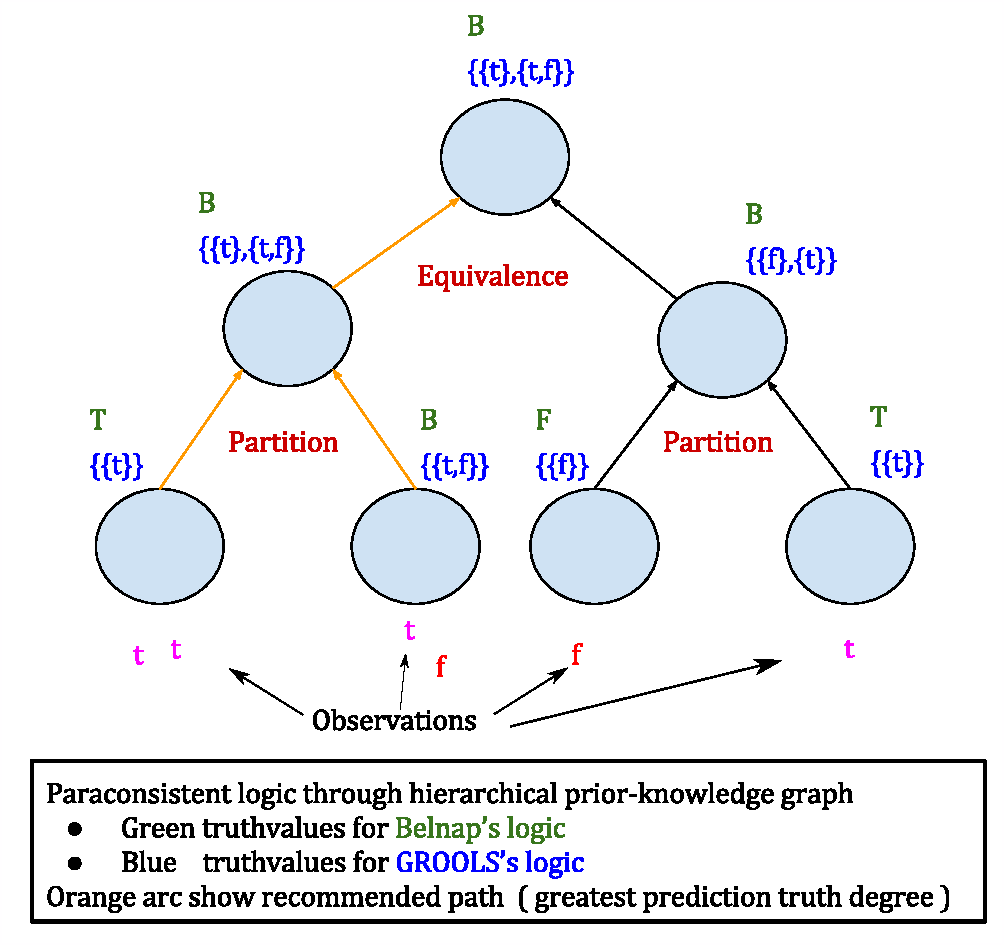
\includegraphics[width=\textwidth]{img/GROOLS_vs_belnap_2.pdf}
    \caption{  }
    \label{fig:grools_belnap_2}
\end{shadedfigure}

\subbibliography
\end{refsegment}